\documentclass[9pt,twocolumn,twoside,lineno]{pnas-new}
% Use the lineno option to display guide line numbers if required.

\templatetype{pnasresearcharticle} % Choose template 
% {pnasresearcharticle} = Template for a two-column research article
% {pnasmathematics} %= Template for a one-column mathematics article
% {pnasinvited} %= Template for a PNAS invited submission

\title{Conceptualizing and Measuring Resilience to Hazards as Access to Essential Services} %Rethinking Resilience: Access to Essentials} %

% Use letters for affiliations, numbers to show equal authorship (if applicable) and to indicate the corresponding author
\author[]{Tom M. Logan}
\author{Seth D. Guikema}

\affil{Industrial and Operations Engineering, University of Michigan, Ann Arbor, USA}

% Please give the surname of the lead author for the running footer
\leadauthor{Logan} 

% Please add here a significance statement to explain the relevance of your work
\significancestatement{
Please add here a significance statement to explain the relevance of your work
}

% Please include corresponding author, author contribution and author declaration information
\authorcontributions{T.L \& S.G devised the approach. T.L collected and analyzed the data, and wrote the paper.}
\authordeclaration{The authors declare no conflict of interest.}
\correspondingauthor{\textsuperscript{*}Correspondence should be emailed to tomlogan@umich.edu}

% Keywords are not mandatory, but authors are strongly encouraged to provide them. If provided, please include two to five keywords, separated by the pipe symbol, e.g:
\keywords{Resilience $|$ Climate change $|$ Communities $|$ Natural Hazards $|$ Urban} 

\begin{abstract}
Despite the extensive discussion surrounding resilience to climate change and natural hazards, operationalizing the concept to enable communities to improve has remained challenging. 
The two dominant approaches to community resilience focus on either assessing community capacity or measuring infrastructure functionality. 
While both remain useful, they have several limitations that means they do not capture important changes within a community following a disaster. 
Nor do the current conceptualizations consider access to essential services or how access is impaired by hazards. 
Given that services such as shelter, food, power, transportation, education, employment, and healthcare are integral to a community’s well being, access to such services is intrinsic to community resilience. 
We propose a new conceptualization of urban resilience that is based on access to essential services together with a way to measure the resilience of a community based on this conceptualization. 
We demonstrate, using two illustrative examples from the impact of Hurricanes Florence and Michael on Wilmington, NC, and Panama City, FL, how decision makers and planners can use this framework to visualize and quantify interventions that increase the resilience of our communities, in a manner that is equitable. 
\end{abstract}

\dates{This manuscript was compiled on \today}
\doi{\url{www.pnas.org/cgi/doi/10.1073/pnas.XXXXXXXXXX}}

\begin{document}

\maketitle
\thispagestyle{firststyle}
\ifthenelse{\boolean{shortarticle}}{\ifthenelse{\boolean{singlecolumn}}{\abscontentformatted}{\abscontent}}{}


\dropcap{A}ccess to services is not something we should take for granted, not before nor after a disaster. Following Hurricane Katrina, residents of New Orleans' Lower 9th Ward were forced to take three buses to reach their nearest grocer \cite{Netter2016-dm}. The 2017 South Asian floods raised fears that thousands of children permanently to dropped out of school \cite{Watt2017-bs}. Even without these disasters, communities throughout the world live within food deserts, health care deserts, and that list goes on. Access to these type of services is important because without it communities cannot function \cite{Winter1997-kc, Logan2017-fr, Dempsey2011-og}, making access to essentials fundamental to their resilience.

As cities urgently need to build their resilience, operationalizing resilience is among today's most impactful research questions \cite{Caldarice2019-tv}. 
Measuring resilience allows us to estimate and compare the effect of interventions and policy changes, as well as target vulnerable communities. 
However, claims including that "resilience is a poorly defined concept not yet operational for policy and management" \cite{Klein2003-lc, Woolf2016-vm}, result from frustration at the challenge.
However, this thinking fails to appreciate that resilience is multidimensional and should be quantified as such. 
It has become conceptual fuzzy \cite{Caldarice2019-tv} and often used as a boundary object because of its malleability \cite{Meerow2016-definingRes}. 
This should not be lost.
Rather, we should disregard the expectation that we can quantify resilience with single metric \cite{Levine2014-je} and seek approaches that will complement one another.

One existing approach to operationalize resilience uses indicators of community capacity. Motivating this approach is the definition of resilience as the ability of a system to respond and recover from disasters. Indicators for this capacity include aspects of social vulnerability (e.g. demographic factors, wealth, and social capital), infrastructure (e.g. building codes, construction practices, and number of amenities), hazard exposure (e.g. risk zones, protective measures), and hazard planning (e.g. governance factors). 

Infrastructure resilience is the other major approach currently used and focuses on a system’s ability to maintain or quickly restore desired functionality. This approach focuses on a specific infrastructure’s (e.g. electricity) ability to withstand a disturbance and quickly repair any damages to restore full system function. This, too, is an essential tool for resilience assessments, 

Although both community capacity indicators and infrastructure functionality measures are useful for our understanding of resilience, there are limitations on their ability to provide actionable insight for building resilience. The indicators provide an understanding of community capacity, preparedness, as well as need. However they provide no information on how a community responds following a hazard’s occurrence. Infrastructure functionality, on the other hand, is essential for assisting the restoration of these networks, but it is not focused on the community served and is independent of the residents’ needs. Neither approach captures how a community can ensure essential services are available to all residents. We propose the access to essentials (ATE) resilience framework as a way of addressing these limitations, complementing and integrating the existing approaches to community resilience, and providing actionable insight to communities trying to build their resilience. 

A further risk with indices is that few are empirically validated \cite{Bakkensen2016-ht}. Another approach, in line with capturing functionality are the tools developed by MCEER \cite{Vugrin2010-vy}. These take a persistence perspective on resilience, considering the system’s robustness and speed of recovery, and are useful for infrastructure systems. While these are important inclusions within the resilience analyst’s suite of tools, the dimension of urban resilience left without quantification relates to the functioning of a community’s essential services. Following an emergency, such as Hurricane Katrina, how many months or years must people go without reasonable access to food?


\section*{Access to essentials}
Accessibility to services in urban areas is crucial for a community’s vitality, livability, and cohesion \cite{Dempsey2011-og, Talen2003-dc}. Residents need services such as education, healthcare, food, and recreation on a regular basis \cite{Dempsey2011-og, Winter1997-kc, Talen2003-dc}. Access to these services for residents is therefore an essential function of a community, both before and after a disruption. Therefore, we propose an approach to measuring resilience based on access to services.

The access to essentials resilience framework we propose measures the distance of residents within a community to their nearest operational essential services. As services shutter and reopen following a disruption we can evaluate how many people are affected, the robustness, the speed of recovery, and the demographics of residents most affected. This spatially explicit approach identifies where and who requires attention from emergency responders. The approach also encourages intervention to reduce service (such as food) deserts, both before and after a hazard so to strengthen the community and reduce inequity.

Improvements in data availability and computational power mean that accurate service proximity can be determined for a community \cite{Logan2017-fr}. Real-time information sharing means that service provision can be measured during and after a natural hazard occurrence. This can be used to guide emergency response as well as short-term and long-term recovery and development. 

The access to essentials resilience framework involves: 
\begin{enumerate}
    \item Engaging the community 
    \begin{enumerate}
        \item Establish which services are essential
    \end{enumerate}
    \item Measuring accessibility \begin{enumerate}
        \item Identify the locations of each service/facility within the region
        \item From each block within the region, determine the network distance to each location
        \item For each block, determine the distance to the nearest operational facility
        \item Map the distances to nearest service (Figure \ref{fig:fig1}a)
        \item Plot the distribution of nearest distances (Figure \ref{fig:fig1}b)
    \end{enumerate}
    \item Monitoring the impacts from a hazard
    \begin{enumerate}
        \item Update the distance to nearest services as facilities open and close
        \item Construct the resilience curve showing how residents' access changes over time (Figures \ref{fig:fig1}c, \ref{fig:cdf_to_res})
        \item Intervene to build resilience (Figure \ref{fig:haz_cycle})
    \end{enumerate}
    \item Evaluating equality (Figure \ref{fig:equality})
    \begin{enumerate}
        \item Differentiate residents based on demographics or vulnerability scores
        \item Evaluate how the access for these various groups compares
        \item Identify vulnerable areas to which to provide additional services and improve equity.
    \end{enumerate}
\end{enumerate}

\begin{figure*}
    \centering
    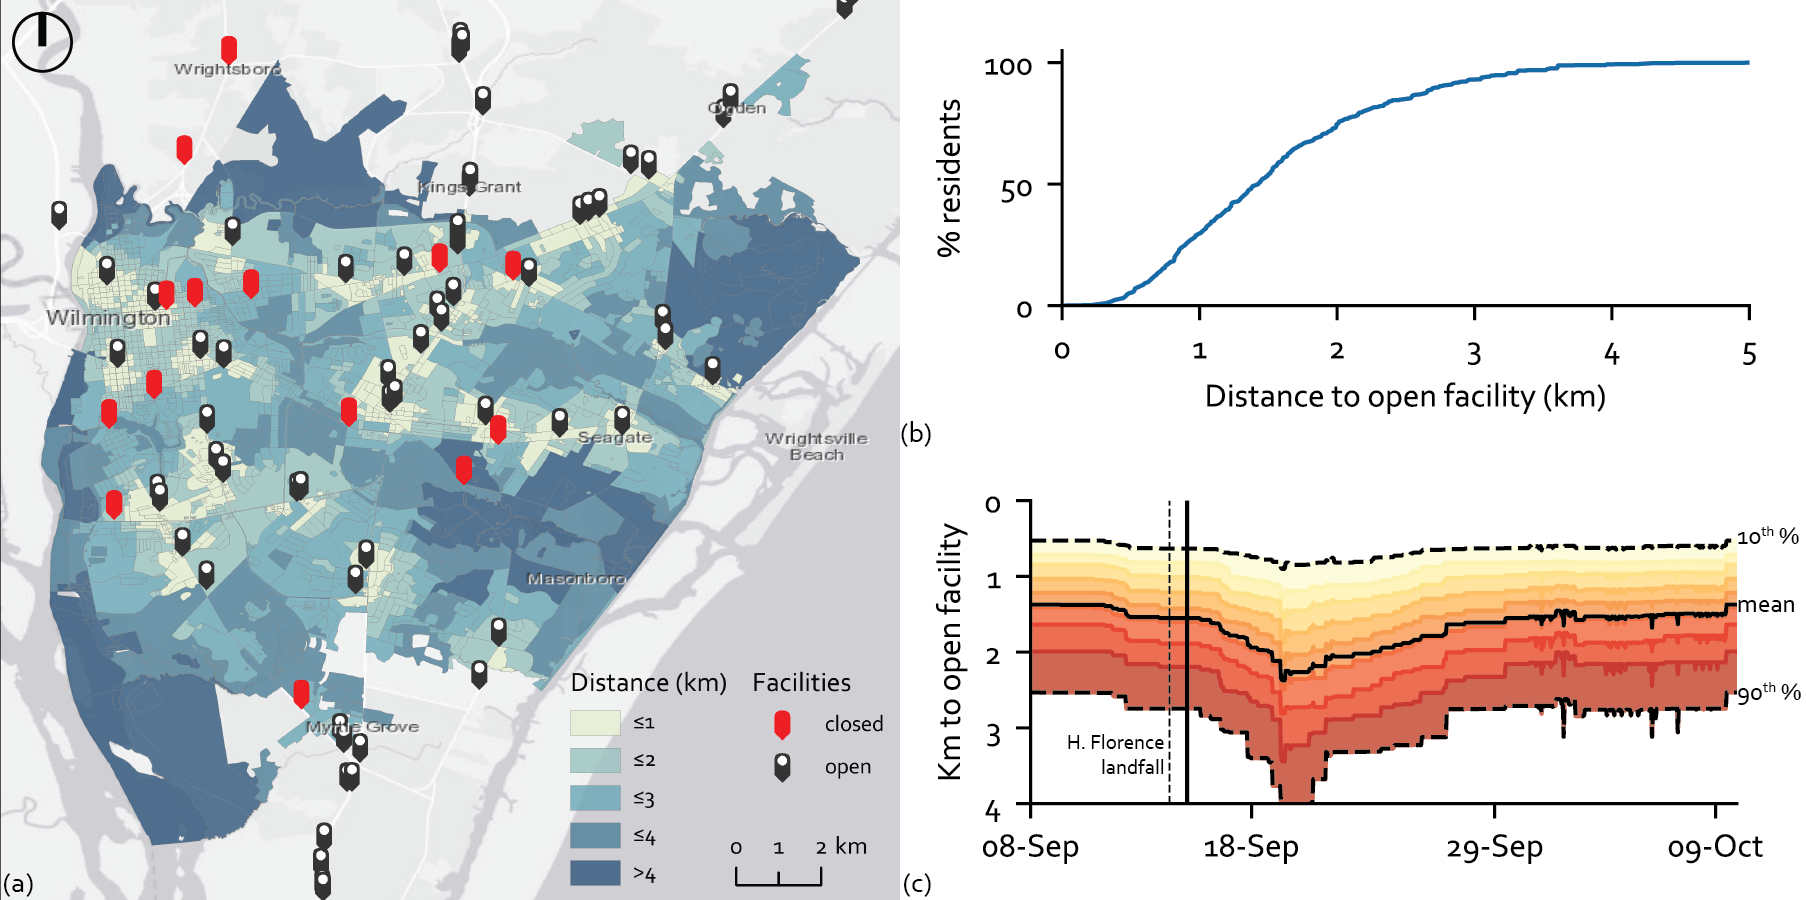
\includegraphics[width=\linewidth]{report/fig/Figure_1.png}
    \caption{This is an example of the access to essentials framework can be used. This is the case of service station access in Wilmington, NC on the 15th of September, 2018. (a) The map of distance to nearest operational service, (b) the cumulative distribution function showing how many residents are closer than “x” to their nearest operational service, and (c) the resilience curve showing how the distribution in access changes over time.
    }
    \label{fig:fig1}
\end{figure*}

%%%%%%%%%% How does this integrate the existing methods?
This approach to quantifying urban resilience satisfies both the persistence and transformation perspectives of resilience by focusing on the functioning of the system, rather than the system’s components \cite{Holling1997-rq}. Rather than returning to a preexisting state, we encourage quickly restoring and improving the functionality. In a resilient urban system, this functionality is the ability of residents to access services they need on a daily basis. In the following section, we discuss how this approach can be used to improve decision making for communities during each stage of the hazard cycle. 

While this approach is dependent upon the facilities in the system, the focus is on the utility of the system for the residents, rather than the system's state and therefore improving the utility of the system can be done either through returning to the previous state or by transforming the system. 




%%%%%%%%%% Equity and targeting vulnerability
A further improvement integrates this approach with measures of need and social capacity. Criticism of approaches such as \cite{Bruneau2006-xc} include that it fails “to capture antecedent social factors that occur at the most local levels or to account for the vulnerability or resilience of the natural environment” \cite{Cutter2008-xv}. While we reiterate that quantifying resilience will likely require more than a single measure \cite{Levine2014-je}, we can integrate social characteristics such as race, income, poverty status, or education into our assessment and evaluate access to vulnerable groups (this is done in \cite{Logan2017-fr} and (green space paper)). However, as with determining thresholds, community indicators and characteristics must be community specific because resilience itself is place-based and community specific. 

%%%%%%%%%%%% Transformation
A further advantage is that this approach encourages transformation both before and following a disruption to improve the equity in our communities. Resilience is often cited as limited for being inherently conservative by promoting the return to pre-existing conditions \cite{Normandin2019-hp, I_Sudmeier-Rieux2014-lc, MacKinnon2013-nx}. This is rooted in Hollings original definition of resilience being resistance to change \cite{Holling1973-wb}. By assessing gross distance, rather than change compared to initial distance, our approach addresses this limitation. This way, it is apparent to decision makers what the existing conditions are, particularly if they are undesirable. Decision makers should be aware of existing food, and other amenity, deserts. When discussing the motivation for opening the only grocery in the New Orleans’ Lower 9th Ward, the owner said, “This is the United States of America. You should not have a hardship like that you have to endure.” He was referring to the three bus journey to the nearest grocery store (How one man single-handedly opened th...). Claims along the lines that people have “grown used to” these abysmal conditions, fail to value the importance of equity and community sustainability for resilience to future events \cite{Dempsey2011-og, Pantelic1991-qu}. Instead, reconstruction must improve residents’ stand of living \cite{Pantelic1991-qu}. Communities are resilient if they are resilient in the long-term; they need to improve their practices and adaptive capacity \cite{Saunders2015-uz}. This requires that operationalizing the concept needs to not simply promote a bouncing back, but a bouncing forward.

%%%%%%%%%%% integrating spatial planning

Urban resilience requires a rethink of how cities are designed, planned, managed, and lived in (Caldarice et al. 2019). To achieve this, our resilience approach must integrate seamlessly into spatial planning. In the remainder of this paper we propose and demonstrate one that does.


This approach integrates spatial planning into the resilience discourse. Although land use planning has long been touted as among the most effective tools for reducing exposure and sensitivity to extreme events \cite{Brunetta2019-ki, Campbell2006-in, Hurlimann2012-uj} (see examples \cite{Logan2018-xj, Anderson2018-hr}), there has been little attempt to actually integrate climate protection and spatial planning in practice \cite{Barnes2017-xf}. This approach brings spatial planning to the forefront of resilience and vulnerability assessment by clearing linking urban changes, social sustainability, and urban resilience.



	Scholars agree that, to-date, the integration of climate protection with spatial planning seems to have taken place mainly at the level of rhetoric and principle, and there are actual challenges in translating these good intentions into practice (Barnes and Nel 2017; Carmin et al. 2012)
		- This methodology is a solution
		- It clearly describes the link between urban changes and adaptation



%%%%%%%%%%%% Access thresholds
The cumulative distribution functions give us the ability to ask what percent of residents live within a sufficient distance of any service. However, there is no consensus on the optimal distance for access \cite{Dempsey2008-hr}. Therefore, the thresholds must be place and service specific and determined by engaging with the communities \cite{Pantelic1991-qu}. This threshold, as with resilience itself, would be normatively indexed, that is, it is an arbitrary and evolving standard of acceptability (analogous to the poverty line, which is geographically specific) \cite{Constas2014-ui}. Regardless of whether a threshold is used, the distribution should still be presented as without it, vulnerable residents can be, and often are, overlooked \cite{Logan2017-fr}. This is especially important given that poverty lies at the root of disaster vulnerability \cite{Pantelic1991-qu}.


\begin{figure*}
    \centering
    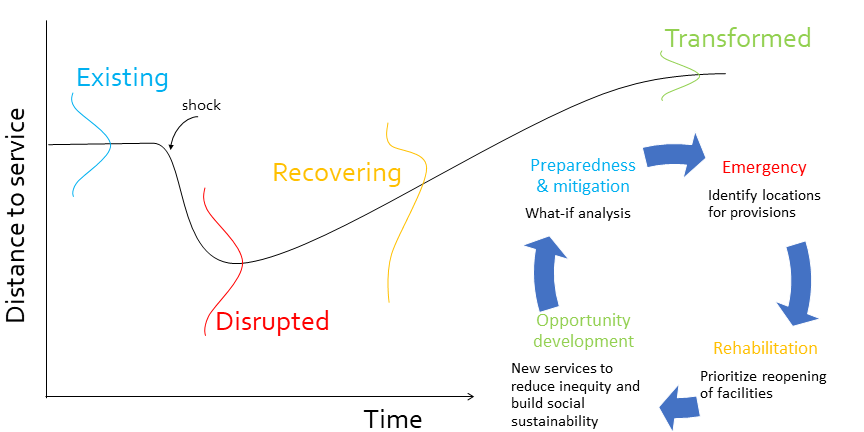
\includegraphics[width=0.8\linewidth]{report/fig/Figure_2.png}
    \caption{Idealized resilience curve }
    \label{fig:haz_cycle}
\end{figure*}

\section*{Extensions}
We argue for considering access to essential services as a measure of resilience on the basis of that access is integral to a community's function.
However, currently we present proximity to services. 
Access, in an urban service context, is comprised of proximity, availability, acceptability, affordability, adequacy, and awareness \cite{Saurman2016-gj, Penchansky1981-qh}. 
Additional advances to using access to quantify resilience need to explore ways to include the additional dimensions, especially affordability and capacity.
This would serve as valuable extensions to the framework.
Nevertheless, proximity is a necessary component for access to services and provides insight into the resilience of a community. 

This approach is suitable for immediate integration into all phases of the hazard cycle. 
Measuring proximity is now practicable and there is real-time information about facility closures. 
Improvements at the implementation level include reliable methods for reporting actual and estimated facility closures and openings. 
These improvements reflect the supply side. 
Improvements to understanding demand include furthering our understanding of the spatial distribution of residents during a disaster.
Integrating cell phone data provides the potential to understand where people have evacuated from, and therefore where emergency supply services should be targeted. 
In the meantime, actionable insight can still be gained from using this approach for emergency response and improving resilience, as we now demonstrate.

\section*{Illustrative examples}
\subsection*{Overview and scope}
We now present two illustrative examples focused on Wilmington, North Carolina, and Panama City, Florida as in late 2018 they were respectively struck by Hurricanes Florence and Michael. 
The example demonstrates how the access to two services (grocery stores and service stations) changes during the period of the hurricane. 
Specifically, we seek to 1) understand the spatial extent of service disruption so service-poor residents can be identified, 2) assess the resilience of the community as a result of these hazards. 
Note that our use of grocery stores and service stations is for demonstration purposes; In practice, determining the essential services as well as the desirable proximity requires stakeholder engagement within each community. 

Wilmington, North Carolina is located on the southeastern North Carolina coast (Figure S2a).
It has a population of approximately 120,000 people, with residents living between the Cape Fear River and the Atlantic Ocean. 
Hurricane Florence made landfall slightly east of Wilmington in the early hours of September 14, 2018, as a Category 1 hurricane. 
On September 7, a week before landfall, the state governor declared a state of emergency, and on September 10 issued a mandatory evacuation order. 
Due to the hurricane’s slow movement, it resulted in heavy rainfall beginning September 13, and coupled with strong storm surge, this resulted in heavy flooding. 

By contrast, Panama City, Florida, has approximately 37,000 residents, and is located along the Emerald Coast of the Florida Panhandle (Figure S2b). 
Hurricane Michael made landfall 40km SouthEast of Panama City as a Category 4 hurricane on October 10. 
While Hurricane Florence was notable for its rainfall, 
Hurricane Michael caused catastrophic damage due to extreme winds (being the strongest to hit the USA since 1992 with winds up to 208 km/h or 129 mph) and storm surge. 
A state of emergency was declared on October 7 and mandatory evacuation by the morning of October 9 was declared on October 8.

\begin{figure}
    \centering
    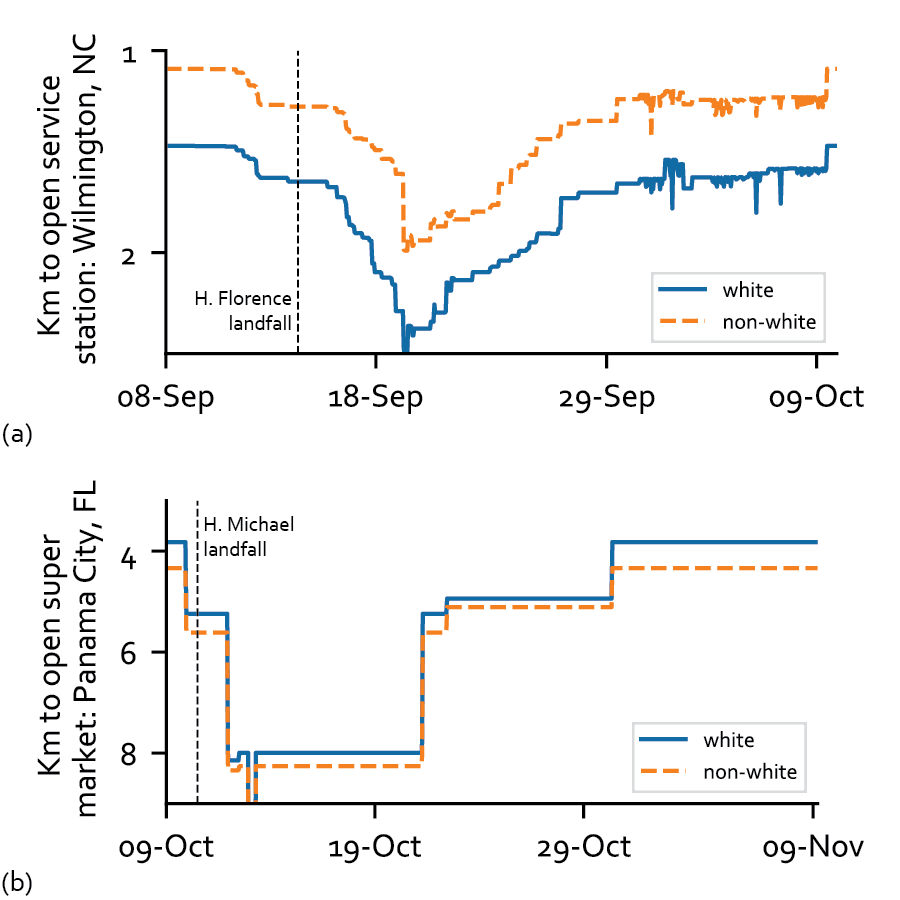
\includegraphics[width=\linewidth]{report/fig/Figure_3.png}
    \caption{Describe}
    \label{fig:equality}
\end{figure}

\subsection*{Inputs}
For this illustrative example we present the access to grocery stores and service stations before and following the hurricanes. 
Service locations were determined using GasBuddy  and supermarkets were identified manually using Google Maps.
Access to these services was calculated at the US census block (neighborhood block) level and shapefiles were sourced from xx. 
The Open Street Map street network was downloaded from xx. 
The distance from each block to all services was calculated using the Open Source Routing Machine (OSRM) using the approach described in \cite{Logan2017-fr}. 
Facility closure was recorded from GasBuddy, Twitter, and the supermarket websites.

\subsection*{Results}
Presented earlier, to introduce the concept, Figure \ref{fig:fig1} shows the access to service stations in Wilmington, NC. The map (a) and cumulative distribution function (b) show the distance of residents to their nearest operational station on the 15th of September, one day after Hurricane Florence made landfall. Figure \ref{fig:fig1}c  shows the resilience curve of proximity to operational station, with the distribution of residents’ access shown by the bands.

Figure 6 shows the access to supermarkets in Panama City, FL. Supermarket access in Wilmington, NC and service station access in Panama City are presented in Appendix A. 

We demonstrate the difference between considering resilience as the percentage of operational facilities versus whether residents have sufficient access with Figure 7. Figure 7 shows the resilience curve of sufficient access (determined by being closer than 800 meters [½ mile] \cite{Talen2003-dc}) to a supermarket, as well as the percentage of operational facilities. This difference is noteworthy because it highlights presenting the state of the system versus the utility derived from the state of the system. Considering resilience in terms of utility also means that transformation is possible because the intention is to provide access rather than return the system to its prior state.

Because determining a suitable threshold is both challenging and arbitrary \cite{Dempsey2008-hr}, we continue to show the distribution of proximity. This, as shown on the resilience curves highlights the variation in residents’ access and potentially quality of life. We see that the residents’ with the better access initially, see very little decrease in proximity compared to those in the higher percentiles. By setting a threshold, care must be taken to not ignore the most vulnerable residents (discussed in \cite{Logan2017-fr}).

\section*{Application throughout the hazard cycle}
The access to essentials resilience framework can enhance decision making throughout the hazard management cycle from mitigation to recovery. The cycle (Figure \ref{fig:haz_cycle}) involves preparing for and mitigating potential hazards; response; and recovery, including the immediate rehabilitation and longer term reconstruction, known as opportunity development.

Operationalizing this approach requires real-time information about the functioning of amenities and critical services be known. Much of this is available online (e.g. Twitter) or a reporting system could be implemented at the local government level. During and \textbf{immediately} following a disruption, this would allow responders to identify impacted areas, inform estimates of demand, and allocate resources appropriately. The real-time service access map would support targeted emergency shelter, health care, and supply tents. 

The \textbf{rehabilitation} phase aims at restoring short term and essential basic services \cite{Resendiz-Vazquez2019-ol}. In this phase, given we know which facilities are closed, optimization can be used to prioritize facility reopening to minimize the disruption in access. Longer term amenities, perhaps recreational (although the importance of amenities is specific to each community and culture), can be prioritized in the same manner, as we move into the reconstruction phase.

During reconstruction we should be building back better \cite{Resendiz-Vazquez2019-ol} by not only enhancing protection against future hazards \cite{Platt2019-lx}, but by improving equity and residents’ quality of life \cite{Pantelic1991-qu}. 
This is why this phase is known as “\textbf{opportunity development}” rather than reconstruction restoring existing conditions \cite{Resendiz-Vazquez2019-ol,Pantelic1991-qu}. 
This phase, which converges into future preparedness and mitigation, could take years and requires longer-term thinking about the growth and demographic shifts of the community. 
In this phase, urban planning must be leveraged to encourage desired amenities such as grocery stores to establish in certain locations. 
For example, comprehensive plans can be used to set minimum numbers for food retailers, zoning mechanisms can simplify the regulatory process, and subsidies or other incentives can recruit retailers to in-need areas \cite{Raja2010-cm, Raja2008-wx}. 
The result should be the continued improvement in the quality of life of the residents (Figure \ref{fig:haz_cycle}). 

Finally, during the \textbf{mitigation and preparedness} phase, what-if style analysis can be used to determine the facilities that are most critical in servicing the community. 
This type of analysis can be used to build redundancy or robustness into the system \cite{Wardekker2010-hw}.

\section*{Conclusion}
Operationalizing urban resilience is among the most impactful research questions \cite{Caldarice2019-tv} as cities urgently need to build their resilience. Central to the definitions and perspectives on urban resilience, and resilience generally, is the ability of the system to maintain and restore desired functionality. In an urban system, we argue that the desired function is to provide everyday amenities to residents such as food, health care, and education. However, existing measures of urban resilience do not capture the sufficiency, or lack of, this access. 

We argue that quantifying urban resilience by measuring the quality of access to essential services and how that quality changes over time. This approach focuses on the utility derived from the system, rather than the system’s explicit state, which encourages not only persistence but transformation and improvement. This approach leads naturally to the quantification of co-benefits as by defining resilience in terms of access to essential services, the myriad of public health, quality of life, equity, and sustainability benefits become goals for policy-makers. 

Although this approach is immediately implementable, we caution policy-makers of the dangers of doing so generically. Resilience is place-based and therefore community specific, so the generic application of this tool (and any other quantification of resilience) with the intention of using it for policy, intervention, aid disbursal must be avoided \cite{Levine2014-je}. Rather, the specific circumstances of each community should be understood and engaging that community should inform the priority of each service and what constitutes a sufficient proximity. 

This approach can be used to improve the resilience and quality of life for residents by informing all stages of the hazard cycle from preparation to redevelopment. It shows the distribution of access so to highlight inequity when it is present and encourage equitable transformation. It does not, nor do we claim that it does, capture all of the complexities of the term resilience. A true understanding of which must capture the multi facets deemed important in a community. In an urban system, access to essential services matters and this framework provides a way of quantifying that. Other approaches that capture other important aspects, complement this approach, and collectively offer an understanding of, and way to improve, the resilience of communities.

Rethinking resilience as access to essential services promotes bounding forward, rather than bouncing back. It complements and integrates aspects of both dominant existing approaches to community resilience. By shifting the focus from the simple state of the infrastructure to the utility that the built environment provides, transformation is encouraged to improve access. This naturally enhances adaptive capacity of the community and existing capacity indicators can be used to prioritize vulnerable residents. The access to essentials framework formalizes resilience in a way that enables and encourages communities to build their resilience, equitably. 

% \matmethods{\subsection*{Data}
% We use the Centers for Disease Control and Prevention's (CDC's) 500 cities data 




% }
% \showmatmethods{} % Display the Materials and Methods section

\acknow{TML is funded by a University of Michigan Rackham PreDoctoral Fellowship and this support is gratefully acknowledged.}

\showacknow{} % Display the acknowledgments section

% Bibliography
\bibliography{references.bib}

\end{document}